\documentclass[11pt, a4paper,spanish]{article}
\usepackage[spanish,activeacute]{babel}
\usepackage[utf8]{inputenc}
\usepackage{caratula}
\usepackage[ruled,vlined,boxed,commentsnumbered]{algorithm2e}
\usepackage{graphicx}
\usepackage{fancyhdr}
\usepackage{amsfonts}
\usepackage{amssymb}
\usepackage{amsmath}
\usepackage{hyperref}
\usepackage{float}

%\usepackage[ruled,vlined,boxed,commentsnumbered]{algorithm2e}

% Encabezado y Pie de pagina
\pagestyle{fancy}
\fancyhf{}
%\fancyfoot[L]{\leftmark}
\fancyhead[L]{Ingeniería del Software 1}
\fancyhead[R]{Trabajo Pr\'actico 1}
\fancyfoot[R]{\thepage}


\begin{document}

% ------------ CARATULA ------------
     

        \materia{Ingeniería del Software 1}

        \submateria{1er cuatrimestre 2014}

    \titulo{Grupo 8: \\Trabajo Práctico 1}

%       \subtitulo{}

%       \fecha{9-04-2014}

    \integrante{Cangiani Agustín}{344/09}{cangiani@gmail.com}

    \integrante{Di Alessio Adrian}{631/06}{adrianalejandro86@hotmail.com}

    \integrante{Grosso Daniel}{694/08}{dgrosso@gmail.com}

    \integrante{Livorno Carla}{424/08}{carlalivorno@hotmail.com}
    
    \integrante{Pino Daniel}{556/07}{jdanielpino@gmail.com}

        \maketitle

        \pagebreak
 

% ------------ INDICE ------------

    \thispagestyle{empty}
    \tableofcontents
    \pagebreak


% ------------ ESENARIOS POSIBLES ------------

\begin{section}{Escenarios}
        
\begin{subsection}{Registración de un usuario}

El usuario se conecta a internet con algún dispositivo(pc, tablet, smartphone) y accede a la página
web del sistema de bicicletas de Mar Chiquita. Como el usuario no se encuentra registrado, necesita 
registrarse para poder acceder al servicio. Para lograrlo deberá ingresar su número de D.N.I, si dicho
número no fue registrado, el sistema le pedirá que ingrese una contraseña para proteger su cuenta. En cambio
si dicho número ya estuviese asignado el sistema le informara al usuario que deberá acercarse a cualquier
terminal del servicio para resolver su situación.

Si la registración fue exitosa, el usuario podrá ingresar de forma opcional la siguiente información:
	\begin{itemize}
	\item Nombre y apellido.
	\item Género.
	\item Dirección donde reside.
	\item Edad.
	\item Profesión.
	\item Estado civil.
	\item Correo electrónico.
	\end{itemize}

Luego el sistema le informará que su cuenta ha sido creada, faltando solamente el paso de verificación, donde
podrá acercarse a cualquier terminal con su D.N.I para confirmar la identidad del usuario. Luego de la 
verificación, el usuario estará en condiciones de retirar una bicicleta desde cualquier terminal.

Por otro lado si el sistema le hubiese informado que su D.N.I ya se encuentra registrado, el sistema le pedirá
que vaya a cualquier terminal para verificar su identificación y corregir su situación.
\end{subsection} 

\begin{subsection}{Retiro de una bicicleta}

\end{subsection} 

\begin{subsection}{Devolución de una bicicleta}

\end{subsection}

\begin{subsection}{Chequeo de stock de bicicletas en una terminal}

\end{subsection}

\begin{subsection}{Una estación se queda sin acceso a internet}

\end{subsection}

\begin{subsection}{Falla en la devolución de una bicicleta}

\end{subsection} 

\begin{subsection}{Un día en la empresa de transporte de bicicletas}

\end{subsection}

\begin{subsection}{Un día en el centro de estadísticas}

\end{subsection}
\end{section}
\pagebreak

% ------------ DIAGRAMA CONTEXTO ------------

\begin{section}{Modelo de agentes}
        

\end{section}
\pagebreak
% ------------ DIAGRAMA OBJETIVOS ------------
\begin{section}{Modelo de objetivos}
        \begin{subsection}{Diagrama de objectivos}
La figura \ref{fig:diagrama_objetivos} puede verse el diagrama de objetivos propuesto, que describe todos los objetivos del problema de las ciclovías.

\begin{figure}[H]
        \centering
        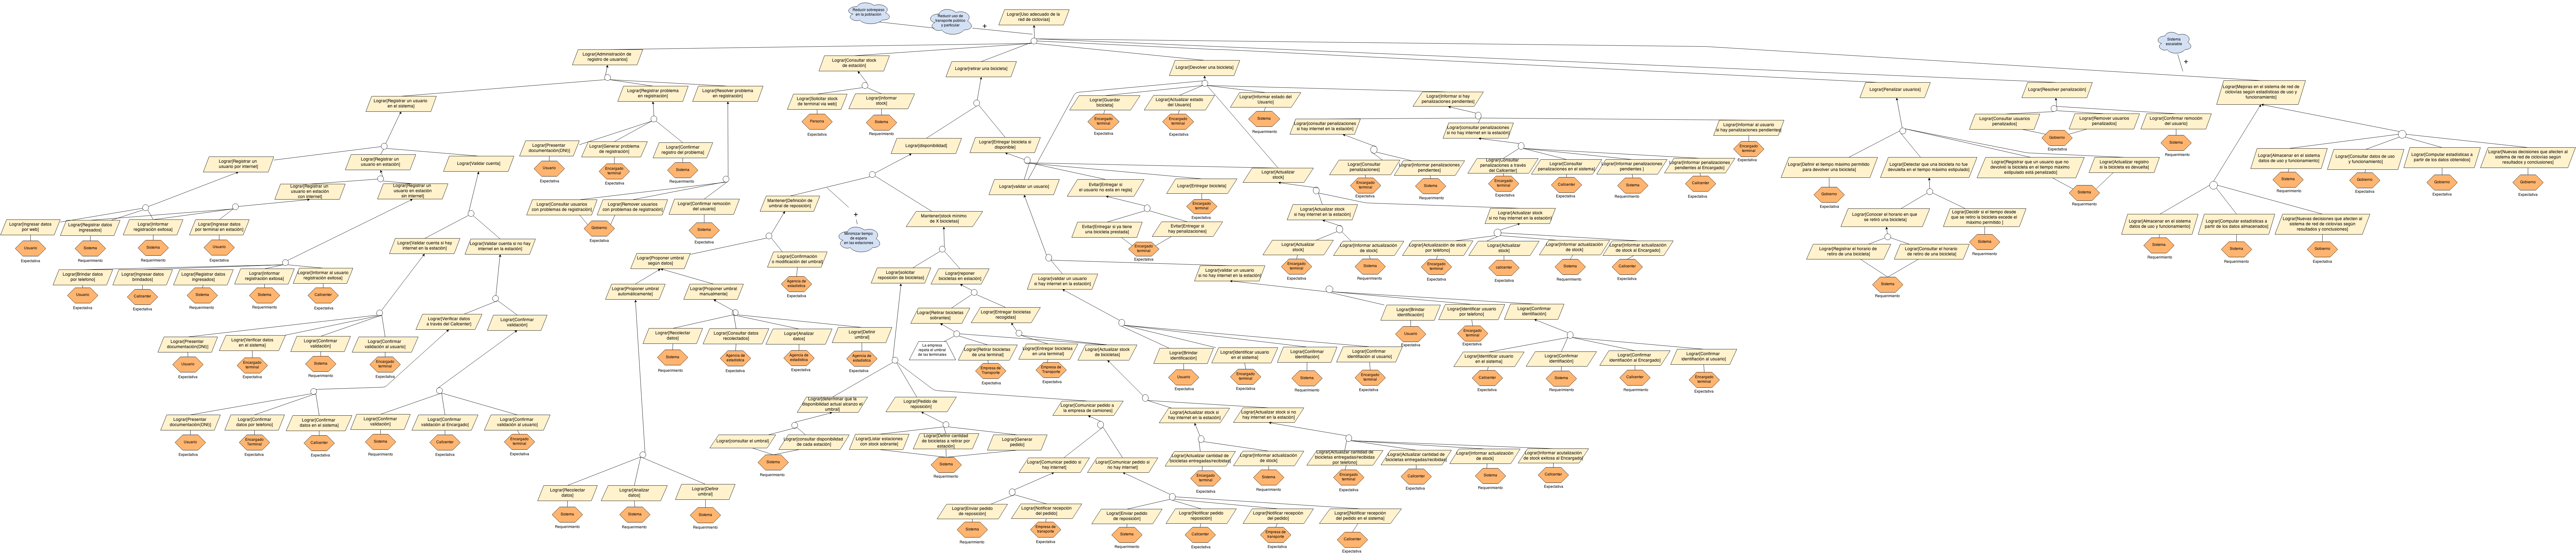
\includegraphics[angle=90,width=\textwidth,height=\textheight,keepaspectratio]{imagenes/diagrama_de_objetivos.png}
        \caption{diagrama de objetivos}
        \label{fig:diagrama_objetivos}
\end{figure}

\begin{figure}[H]
        \centering
        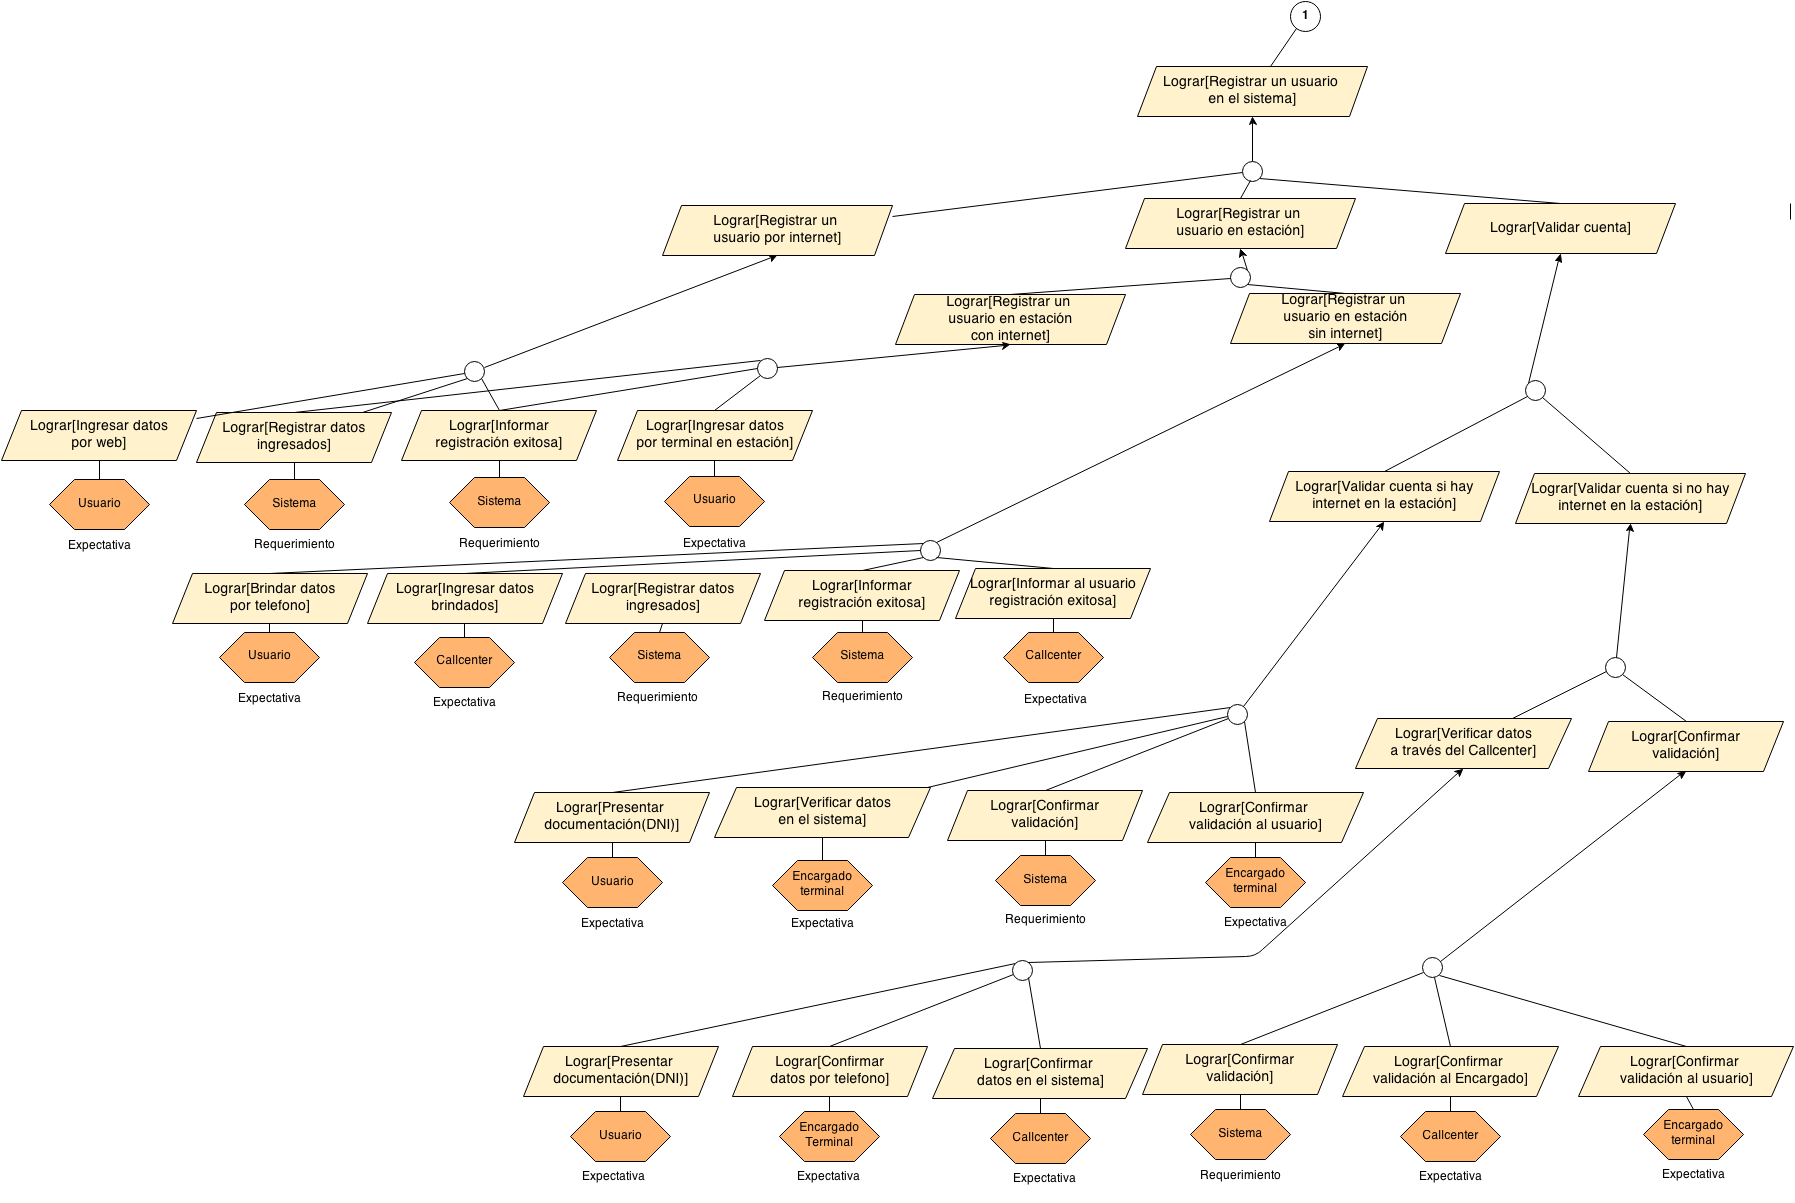
\includegraphics[angle=90,width=\textwidth,height=\textheight,keepaspectratio]{imagenes/do_1.png}
        \caption{diagrama de objetivos - 1}
        \label{fig:diagrama_objetivos_1}
\end{figure}

\begin{figure}[H]
        \centering
        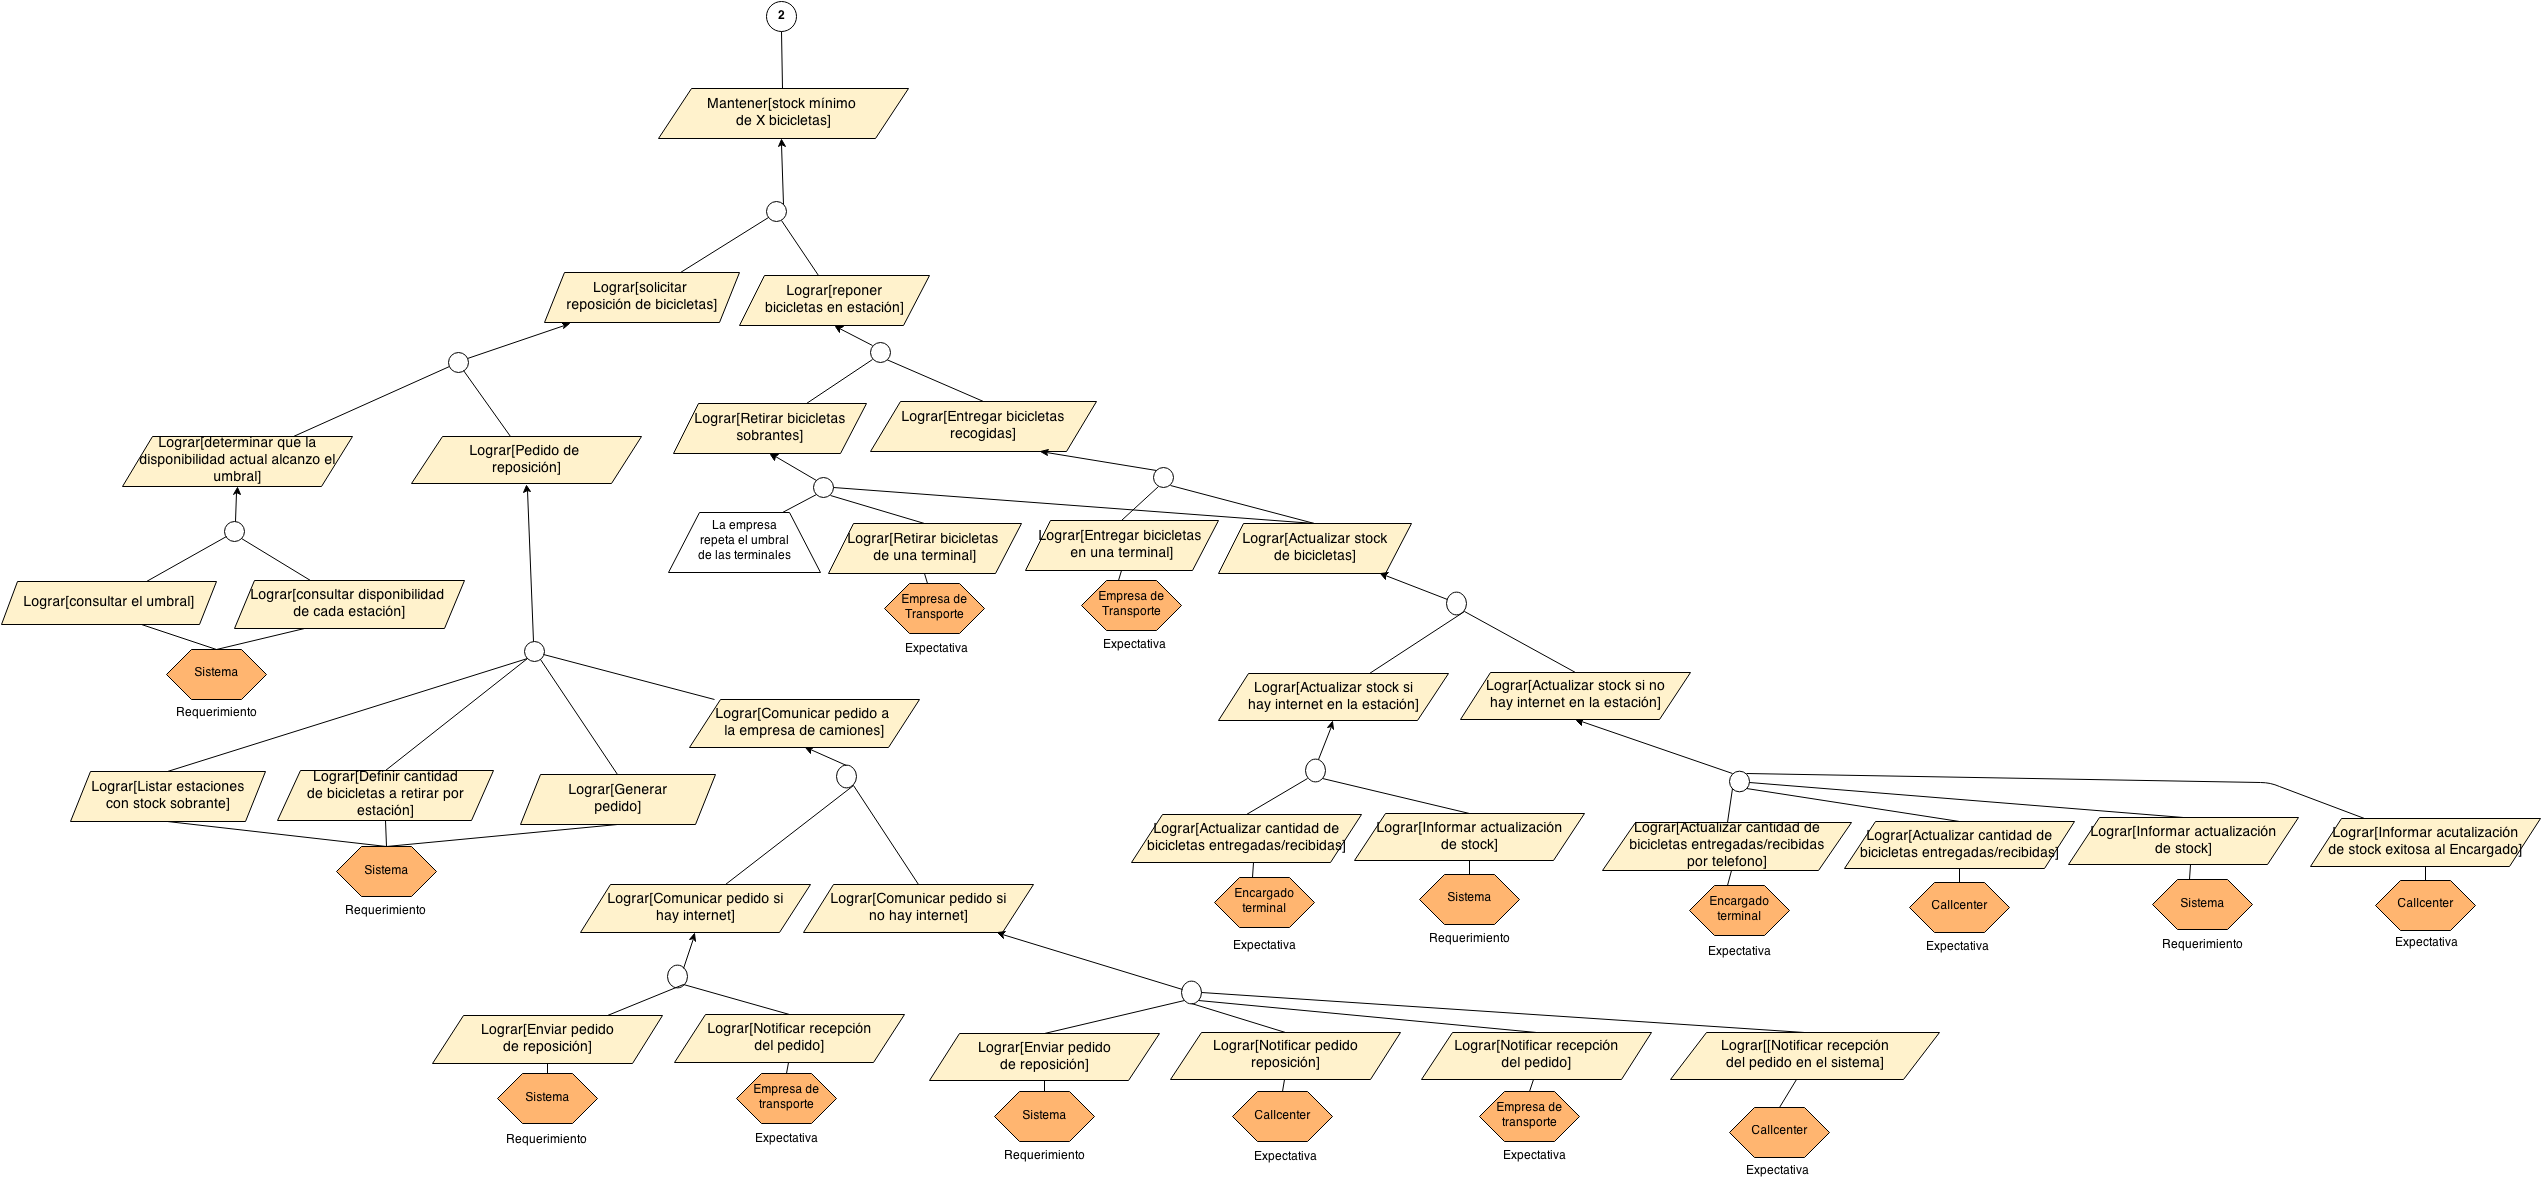
\includegraphics[angle=90,width=\textwidth,height=\textheight,keepaspectratio]{imagenes/do_2.png}
        \caption{diagrama de objetivos - 2}
        \label{fig:diagrama_objetivos_2}
\end{figure}


\begin{figure}[H]
        \centering
        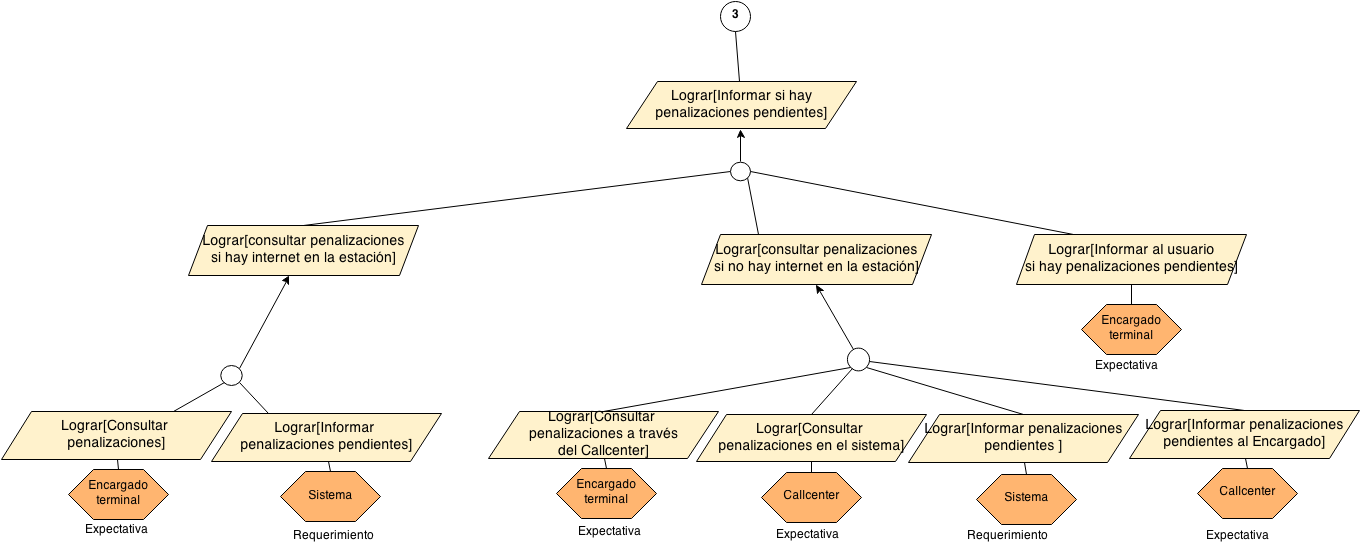
\includegraphics[angle=90,width=\textwidth,height=\textheight,keepaspectratio]{imagenes/do_3.png}
        \caption{diagrama de objetivos - 3}
        \label{fig:diagrama_objetivos_3}
\end{figure}

\begin{figure}[H]
        \centering
        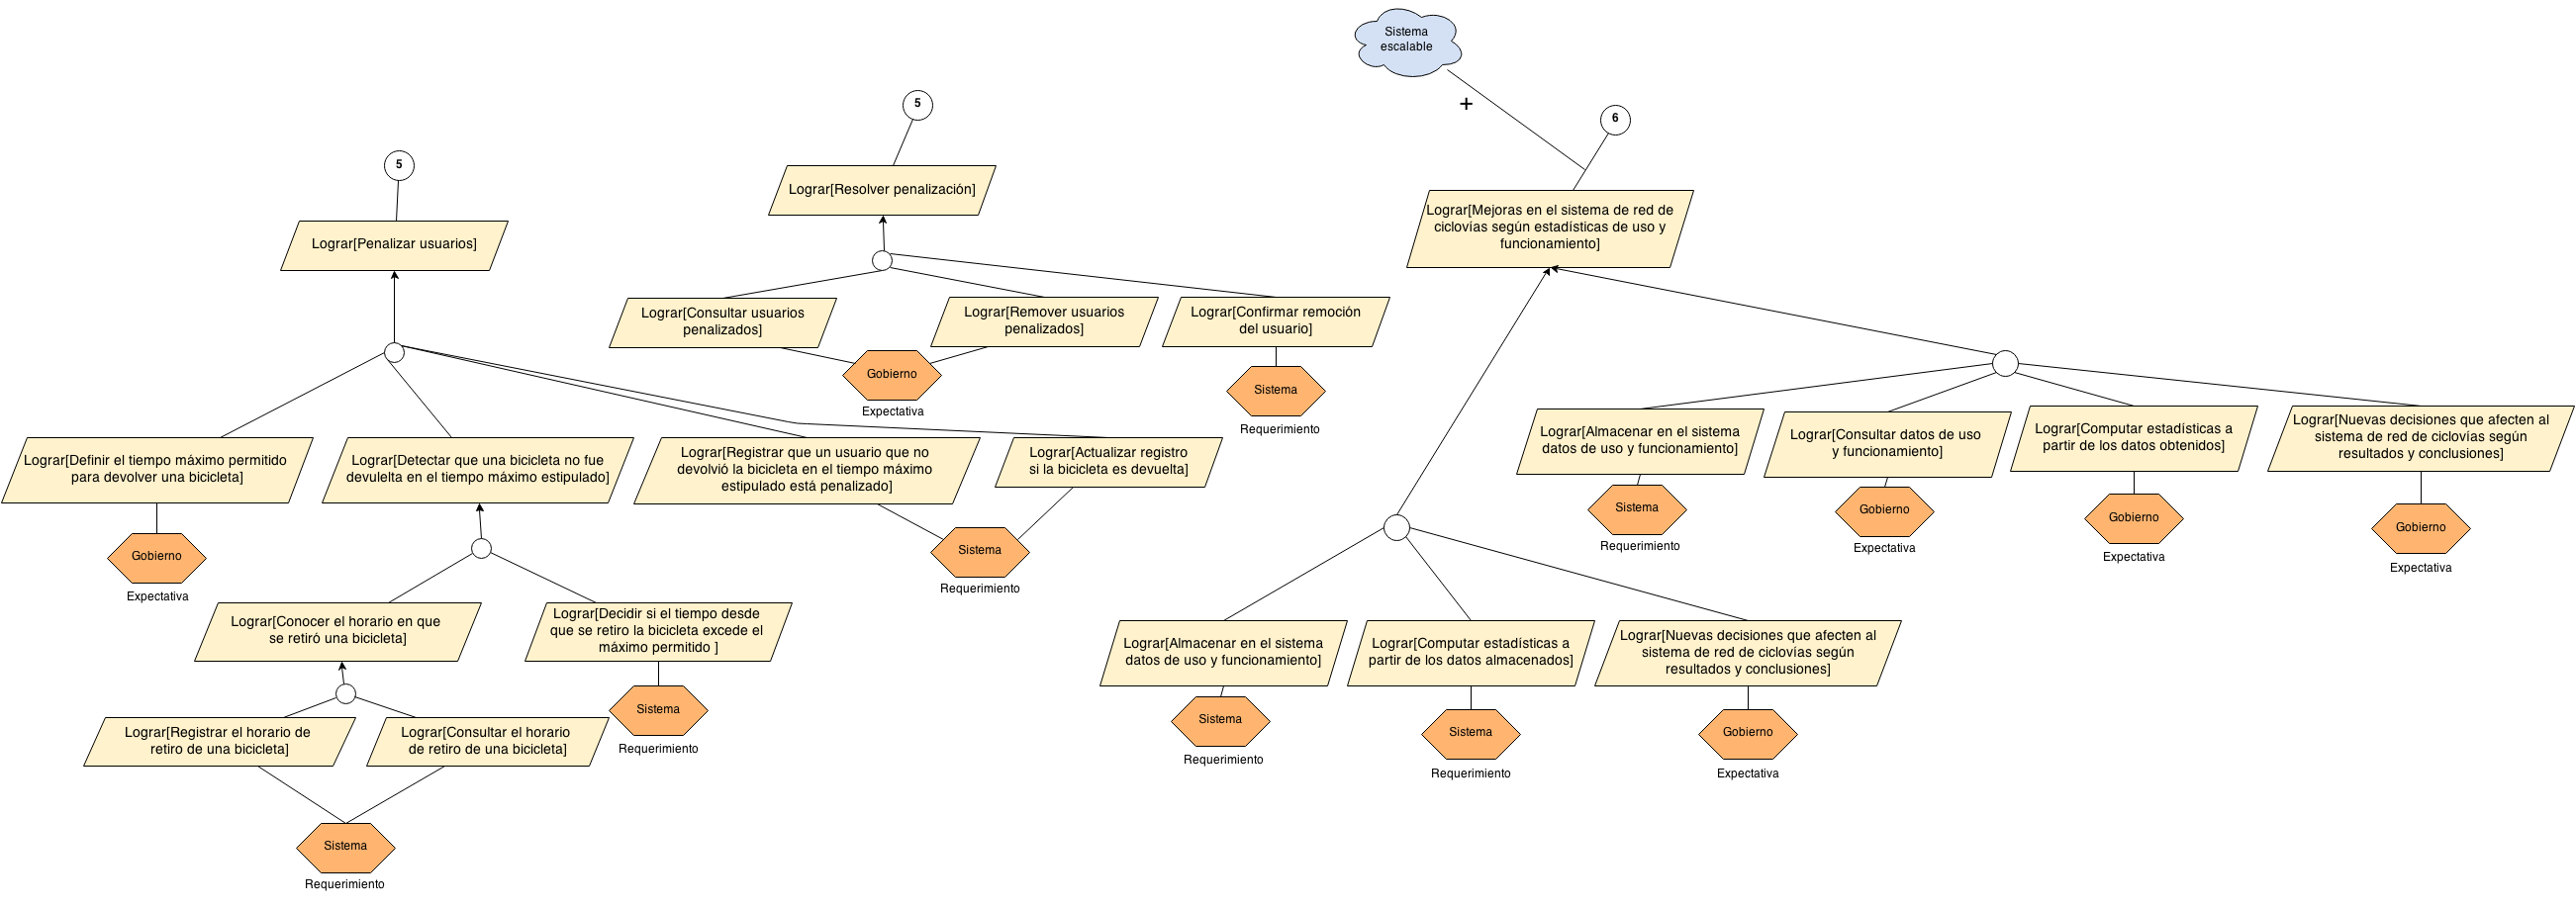
\includegraphics[angle=90,width=\textwidth,height=\textheight,keepaspectratio]{imagenes/do_4-5-6.png}
        \caption{diagrama de objetivos - 4 5 6}
        \label{fig:diagrama_objetivos_4_5_6}
\end{figure}
%\begin{figure}[H]
%	
%	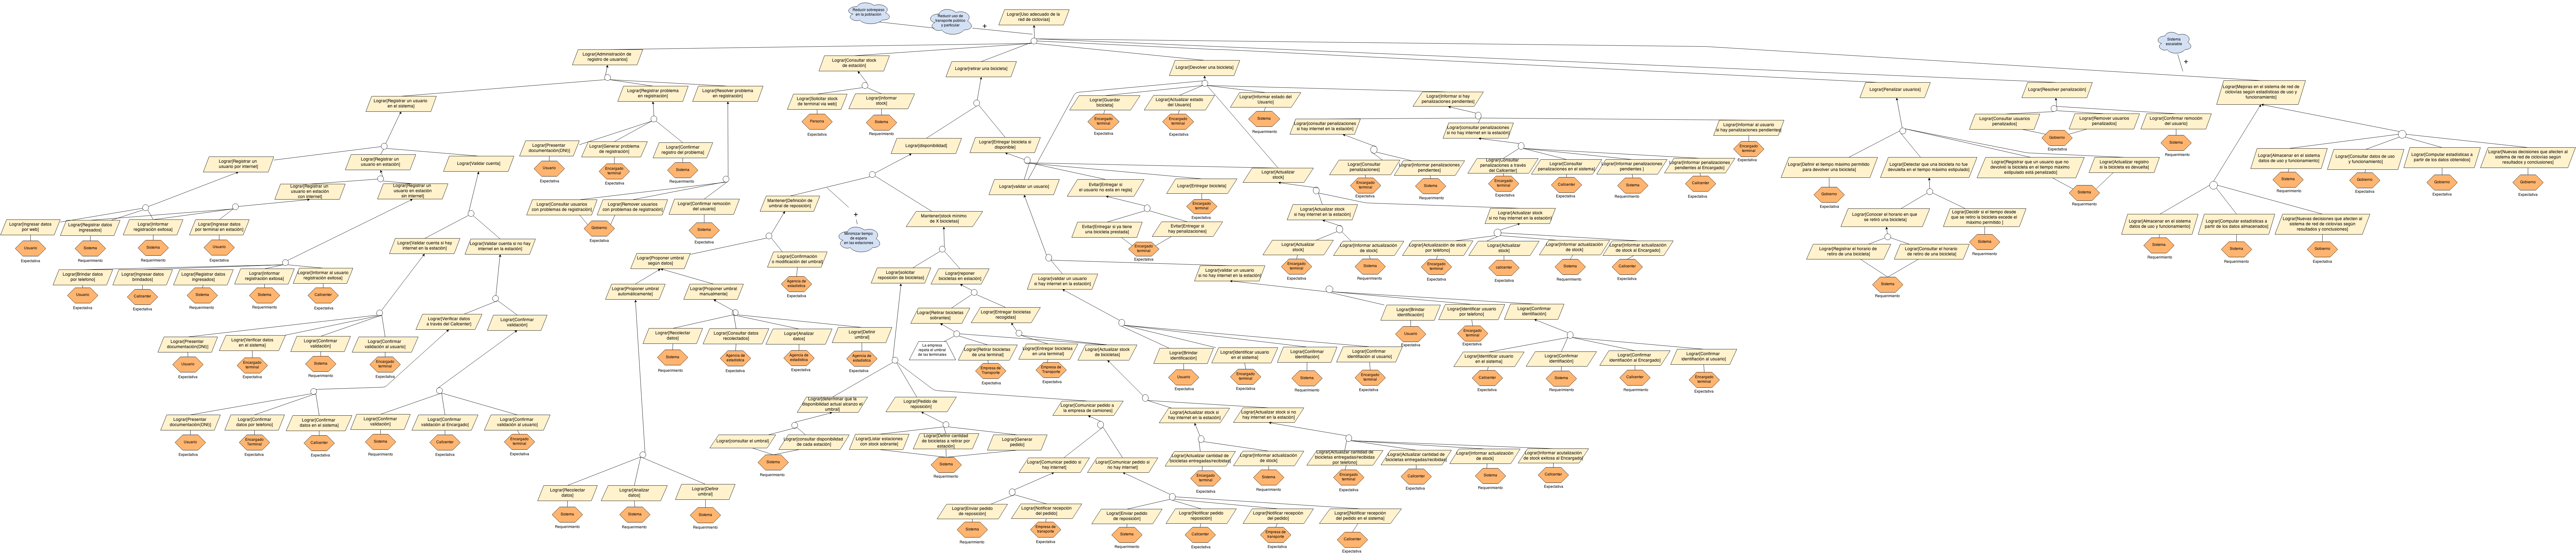
\includegraphics[scale=0.47]{imagenes/diagrama_de_objetivos.png}
%	\caption{diagrama de contexto}
%	\label{fig:diagrama_objetivos}
%
%\end{figure}

\end{subsection}

%\begin{subsection}{Análisis de objetivos}

%\end{subsection}
\end{section}\begin{flushleft}\end{flushleft}

% ------------ REFERENCIAS ------------
    \pagebreak
%    \section{Referencias}
%        



\end{document}